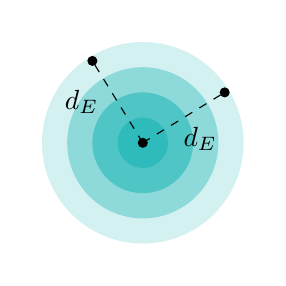
\begin{tikzpicture}[scale=0.8]
    \coordinate (A) at (0,0);
    \coordinate (B) at (1.3,0.8);
    \coordinate (C) at (-0.8,1.3);

    \foreach\i in {0.2,0.4,...,1} {
        \fill[opacity=\i,BlueGreen,rotate around={30:(A)}] (A) ellipse ({2-2*\i} and {2-2*\i});         
      }

    \draw[dashed] (A) -- (B) node [pos=.7, label=below:$d_E$] {};
    \draw[dashed] (A) -- (C) node [pos=.5, label=left:$d_E$] {};

    \draw[fill=black, draw=black] (A) circle (2pt);
    \draw[fill=black, draw=black] (B) circle (2pt);
    \draw[fill=black, draw=black] (C) circle (2pt);
\end{tikzpicture}%
